\chapter{Numerics}

\section{Numerical schemes for the heat equation}

The heat equation is on the form
\begin{equation}
\frac{\partial u}{\partial t}=\mu \grad{^2 u} + K,
\label{heatequation}
\end{equation}
Here K is a constant, and we thus neglect it in the discretization of (\ref{heatequation}).\\

In this project the Cranch-Nicholson method was used to discretize the heat
equation \cref{eq:heat1} in 3D over a finite grid. This method was chosen because
it is unconditionally stable, and it converges in second order in time and
space, as is shown below. \\

The Crank-Nicholson method is based on the equation \cref{integral}, where the trapezoidal rule \cref{trapezoidalrule} is used to approximate the integral on the right hand side. We insert the right hand side of the heat equation in the resulting expression \cref{res}, and use Taylor-expansion to obtain the discretizaion. We use the notation \cref{notations} in the rest of this document.

\begin{equation}
\partial_{x}^{k}u=\frac{\partial^{k}u}{\partial^{}x^{k}},\quad \quad \partial_{t}^{k}u=\frac{\partial^{k}u}{\partial^{}t^{k}} \quad \quad u_{m}^{n+\alpha k } = u(x_{m},t_{n}+\alpha k)
\label{notations}
\end{equation}

\begin{equation}
u(x_m,t_{n+1}) - u(x_m,t_n) = \int_{t_n} ^{t_{n+1}} u_t(x_m,t) dt
\label{integral}
\end{equation}

\begin{equation}
\int_0^k f(t) dt = \frac{1}{2} k (f(0) - f(k)) -\frac{1}{12} k^3 f''(\frac{k}{2}) + ...
\label{trapezoidalrule}
\end{equation}
We thus obtain
\begin{eqnarray}
\label{res}
u_m^ {n+1} &=& u_m^ n + \frac{1}{2} k(\partial_t u_m^n + \partial_t u_m^{n+1}) - \frac{1}{12} k^3 \partial_t ^3 u_m^{n+\frac{1}{2}} + ...\\
&\stackrel{\text{\tiny heat eq.}}{=}& u_m^ n + \frac{1}{2} \mu k(\partial_x^2 u_m^n + \partial_y^2 u_m^n + \partial_z^2 u_m^n + \partial_x^2 u_m^{n+1} + \partial_y^2 u_m^{n+1} + \partial_z^2 u_m^{n+1}) - \frac{1}{12} k^3 \partial_t ^3    u_m^{n+\frac{1}{2}} + ... \nonumber
\end{eqnarray}
Using central differences \cref{centraldiff}, and denoting the step sizes in $x, y, z$ direction by $h, f, g$ respectively gives
\begin{eqnarray*}
u_m^{n+1} &=& u_m^ n + \frac{1}{2} \mu k(\frac{1}{h^2}\delta_x^2 u_m^n + \frac{1}{f^2}\delta_y^2 u_m^n + \frac{1}{g^2}\delta_z^2 u_m^n + \frac{1}{h^2}\delta_x^2 u_m^{n+1} + \frac{1}{f^2}\delta_y^2 u_m^{n+1} + \frac{1}{g^2}\delta_z^2 u_m^{n+1}) \\
  &&- \frac{1}{2} \mu k (\frac{1}{12}h^2\partial_x^4 u_m^n +
  \frac{1}{12}g^2\partial_y^4 u_m^n + \frac{1}{12}f^2\partial_z^4 u_m^n +
  \frac{1}{12}h^2\partial_x^4 u_m^{n+1} + \frac{1}{12}g^2\partial_y^4
  u_m^{n+1}\\
  &&+ \frac{1}{12}f^2\partial_z^4 u_m^{n+1} + \cdots)
  - \frac{1}{12} k^3 \partial_t ^3 u_m^{n+\frac{1}{2}} \\ 
  %&=& u_m^n + \frac{r}{2}(\delta_x^2 u_m^n + \delta_x^2 u_m^{n+1}) + \frac{p}{2}(\delta_y^2 u_m^n + \delta_y^2 u_m^{n+1}) + \frac{q}{2}(\delta_z^2 u_m^n + \delta_z^2 u_m^{n+1}) + \tau_m^n
\end{eqnarray*}
where
\begin{equation}
\delta_{r}^{2}U_m^{n}=\frac{U_{m+1}^{n}-2U_m^{n}+U_{m-1}^{n}}{{\Delta r}^{2}}
\label{centraldiff}
\end{equation}
At this point it may be instructive to use \cref{fig:stencil-numerics} as a guideline.

\begin{figure}[h!]
  \begin{center}
    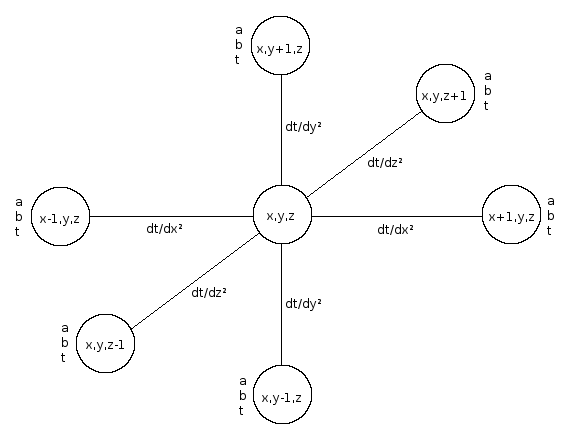
\includegraphics[width=0.7\textwidth]{stencil.png}
  \end{center}
  \caption{Stencil for the Crank Nicolson method}
  \label{fig:stencil-numerics}
\end{figure}

We thus obtain the implicit method for the heat equation
\begin{equation}
u_m^{n+1}-\mu k(\frac{1}{h^2}\delta_x^2 u_m^{n+1}-\frac{1}{f^2}\delta_y^2 u_m^{n+1}-\frac{1}{g^2}\delta_z^2 u_m^{n+1})=u_m^n + \mu k(\frac{1}{h^2}\delta_x^2 u_m^n + \frac{1}{f^2}\delta_y^2 u_m^n +\frac{1}{g^2}\delta_z^2 u_m^n)
\label{crank}
\end{equation}
with truncation error error
\begin{eqnarray}
\frac{\tau_m^ n}{k} &=& -\frac{1}{12} \mu k^2 \partial_t^2 u_m^{n+\frac{1}{2}} - \frac{1}{12} \mu h^2 \partial_x^4 u_m^{n+\frac{1}{2}} - \frac{1}{12} \mu g^2 \partial_y^4 u_m^{n+\frac{1}{2}} - \frac{1}{12} \mu f^2 \partial_z^4 u_m^{n+\frac{1}{2}}\\
&=& \mathcal{O} (k^2 + h^2 + g^2 + f^2)
\label{truncerror}
\end{eqnarray}

Here we have used that $\frac{1}{2}(\partial_x^4 u_m^n + \partial_x^4 u_m^{n+1}) = \partial_x^4 u_m^{n+\frac{1}{2}} + \mathcal{O} (k^2)$. 
The truncation error $\tau_m^n \Rightarrow 0$ as $h,f,g,k \Rightarrow 0$, and the Crank-Nicholson method is consistent for the heat equation. To see if the method converges we perform a von Neumann analysis of the numerical scheme.

\section{Von Neumann analysis of the Crank-Nicholson-scheme}

The von Neumann analysis is based on Fourier analysis, see \cite{aarseth}. The method consist of substituting 
\begin{equation*}
	U_m^n=\xi^n e^{i \beta x_m} \quad \quad  i=\sqrt{-1}
\end{equation*}
in the difference equation and solving for $\xi$.
For the method to be stable it has to meet the condition
\begin{equation}
	\mid{\xi}\mid \leq 1
	\label{stabcond}
\end{equation}

Here we only perform the von Neumann analysis for the one-dimensional heat
equation, giving the expression
\begin{equation*}
\xi^{n+1} e^{i\beta x_{j}} = \xi^{n} e^{i\beta x_j}\left(1-2D\right) + \xi^{n+1}D\left(e^{i\beta x_{j+1}} - 2e^{i\beta  x} + e^{i\beta x_{j-1}}\right) + \xi^{nD}\left(e^{i\beta x_{j+1}} + e^{i\beta x_{j-1}}\right)
\end{equation*}

where
\begin{equation*}
D = \frac{1}{2}\frac{\alpha\Delta t}{(\Delta x)^2}
\label{eq:crank-D}
\end{equation*}

Dividing  by $\xi^ne^{i\beta x_j}$, and using $x_{j+1} = x_j + h$ one obtains    %\href{eq:crank-D}
\begin{eqnarray*}
\xi\left[1-D\left(2\cos{\beta h} - 2\right)\right] &=& 1 - 2D\left(1-\cos{\beta h}\right) \\
\cos{\beta h} &=& 1-2\sin^2{\frac{\beta h}{2}} \\
\xi\left(1+4D\sin^{2}{\frac{\beta h}{2}}\right) &=& 1 - 4D\sin^2{\frac{\beta h}{2}} \\
\xi &=& \frac{1-4D\sin^2{\frac{\beta h}{2}}}{1+4D\sin^2{\frac{\beta h}{2}}}
\end{eqnarray*}
As the maximum value of $\sin^2{x}$ is 1, the methods meets the stability condition \ref{stabcond}.
\begin{equation}
|\xi | = \left|\frac{1-4D}{1+4D}\right|
\end{equation}

Since D is always positive, we get that the Crank-Nicolson
scheme for the heat equation is \emph{unconditionally stable}. In practice it
may happen that the method oscillates if the time steps and space steps do not
fulfill a CFL-condition\footnote{Courant-Friedrichs-Levy condition}.
\\
\\
From Lax' equivalent theorem, which states that a consistent difference scheme will converge if and only if it is stable, the Crank-Nicholson scheme will converge.


%\section{Truncation error in the Crank-Nicolson scheme}

%The Crank-Nicholson method is based on the trapezoidal rule. From the trapezoidal rule the truncation error is represented by
%\begin{equation*}
%\int_0^k f(t) dt = \frac{1}{2} k (f(0) - f(k)) -\frac{1}{12} k^3 f''(\frac{k}{2}) + ...
%\end{equation*}
%Using the formula
%\begin{equation*}
%	u(x_m,t_{n+1}) - u(x_m,t_n) = \int_{t_n} ^{t_{n+1}} u_t(x_m,t) dt
%\end{equation*}
%and approximating the integral by the trapezoidal rule, and abbreviate the notation $u_m^{n+1/2} = u(x_m,t_n+\frac{1}{2} k)$, one obtain
%\begin{eqnarray*}
%u_m^ {n+1} &=& u_m^ n + \frac{1}{2} k(\partial_t u_m^n + \partial_t u_m^{n+1}) - \frac{1}{2} k^3 \partial_t ^3 u_m^{n+\frac{1}{2}} \\
%		   &\stackrel{\text{\tiny heat eq.}}{=}&  u_m^ n + \frac{1}{2} k(\partial_x^2 u_m^n + \partial_y^2 u_m^n + \partial_z^2 u_m^n + \partial_x^2 u_m^{n+1} + \partial_y^2 u_m^{n+1} + \partial_z^2 u_m^{n+1}) - \frac{1}{2} k^3 \partial_t ^3 u_m^{n+\frac{1}{2}}
%\end{eqnarray*}
%Discretizing the double derivative with central differences, and denoting the step sizes in $x, y, z$ direction by $h, f, g$ respectively, gives
%\begin{eqnarray*}
%u_m^{n+1} &=&  u_m^ n + \frac{1}{2} k(\frac{1}{h^2}\delta_x^2 u_m^n + \frac{1}{f^2}\delta_y^2 u_m^n + \frac{1}{g^2}\delta_z^2 u_m^n + \frac{1}{h^2}\delta_x^2 u_m^{n+1} + \frac{1}{f^2}\delta_y^2 u_m^{n+1} + \frac{1}{g^2}\delta_z^2 u_m^{n+1}) \\
% 		  &&- \frac{1}{2} k (\frac{1}{12}h^2\partial_x^4 u_m^n + \frac{1}{12}g^2\partial_y^4 u_m^n \frac{1}{12}f^2\partial_z^4 u_m^n + \frac{1}{12}h^2\partial_x^4 u_m^{n+1} + \frac{1}{12}g^2\partial_y^4 u_m^{n+1} \frac{1}{12}f^2\partial_z^4 u_m^{n+1} ) \\
% 		  &&- \frac{1}{2} k^3 \partial_t ^3 u_m^{n+\frac{1}{2}} \\
% 		  &=& u_m^n + \frac{r}{2}(\delta_x^2 u_m^n + \delta_x^2 u_m^{n+1}) + \frac{p}{2}(\delta_y^2 u_m^n + \delta_y^2 u_m^{n+1}) + \frac{q}{2}(\delta_z^2 u_m^n + \delta_z^2 u_m^{n+1}) + \tau_m^n
%\end{eqnarray*}
%where $r = k/h^2$, $p = k/f^2$, $q = k/g^2$, and $\tau_m^n$ is the truncation error times $k$. The expression for $\tau_m^n$ is
%\begin{equation*}
%\tau_m^n = -\frac{1}{12} k^3 \partial_t^2 u_m^{n+\frac{1}{2}} - \frac{1}{12} k h^2 \partial_x^4 u_m^{n+\frac{1}{2}} - \frac{1}{12} k g^2 \partial_y^4 u_m^{n+\frac{1}{2}} - \frac{1}{12} k f^2 \partial_z^4 u_m^{n+\frac{1}{2}}
%\end{equation*}
%where we have used $\frac{1}{2}(\partial_x^4 u_m^n + \partial_x^4 u_m^{n+}) = \partial_x^4 u_m^{n+\frac{1}{2}} + O(k^2)$. Hence, the truncation error is 
%\begin{eqnarray*}
%\frac{\tau_m^ n}{k} &=& -\frac{1}{12} k^2 \partial_t^2 u_m^{n+\frac{1}{2}} - \frac{1}{12} h^2 \partial_x^4 u_m^{n+\frac{1}{2}} - \frac{1}{12} g^2 \partial_y^4 u_m^{n+\frac{1}{2}} - \frac{1}{12} f^2 \partial_z^4 u_m^{n+\frac{1}{2}}\\
%					&=& O(k^2 + h^2 + g^2 + f^2)
%\end{eqnarray*}

